\subsection{Experimental Methods for Colour Constancy Research}

\begin{citequote}{hurlbert_colour_2007}
\emph{How is colour constancy measured?} With difficulty.
\end{citequote}



CIE 160:2004 \citep{cie_tc_1-52_cie_2004} and \citet{luo_review_2000} provide a comprehensive overview of the different methods which have been used by the \gls{CAT} group:

\begin{itemize}
\item Haploscopic matching
\item Local Adaptation Matching
\item Memory Matching
\item Magnitude Estimation
\end{itemize}


\paragraph{Haploscopic Matching} is the most common technique in this field, and the term refers to experiments which differentially adapt the two eyes and allow an observer to vary attributes of the stimulus presented to one eye such that it in some way matches the attributes of a fixed stimulus shown to another eye. Whilst this is in many ways unnatural, the benefits are that an experiment can be set up so that there is no time interference (the presentations are simultaneous, so memory effects are avoided) and that high precision of match is relatively easily achieved. An assumption is made that the adaptation of each eye is independent.

\begin{figure}[htbp]
    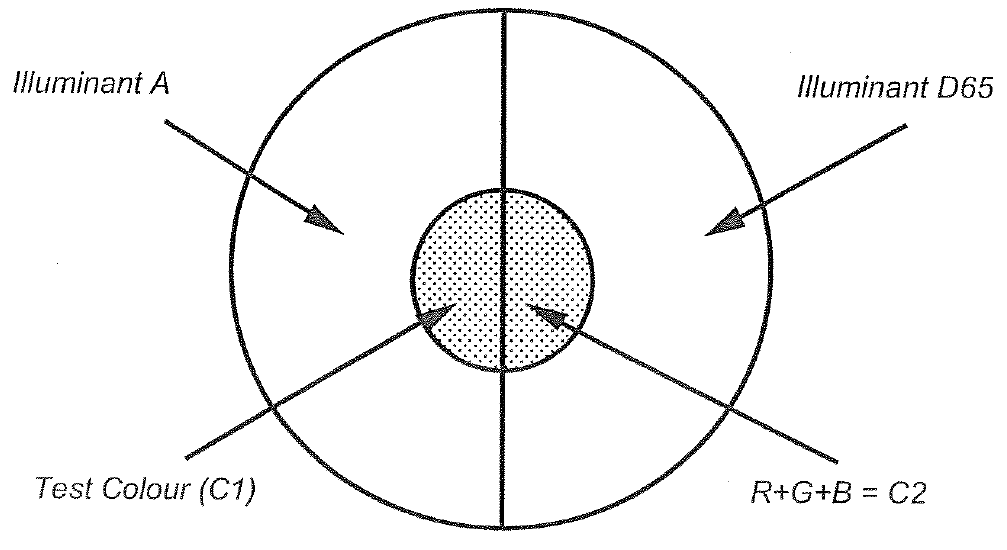
\includegraphics[max width=\textwidth]{figs/LitRev/hapl.png}
    \caption{Figure 11 from \citet{cie_tc_1-52_cie_2004}, showing `A typical viewing condition used in the haploscopic matching experiment'.}
    \label{fig:hapl}
\end{figure} 


\paragraph{Local Adaptation Matching} can be considered as a variation of haploscopic matching where instead of differing adaptational stimuli being presented to each eye, differing adaptational stimuli are presented to different parts of the same eye (spatially distinct areas of the same retina). The assumption here is that there is minimal intra-retinal interaction. MacAdam's 1956 study \citep{macadam_chromatic_1956} epitomises this technique. This experimental technique requires that observers minimise eye movement, in order to maintain spatially distinct adaptation.

\paragraph{Memory Matching} has traditionally been performed by training observers to communicate colour sensation through the Munsell system notation \citep{helson_object-color_1952,lam_metamerism_1985} and then asking observers adapted to different ambient lighting to describe set real objects using such notation. This technique is not much used due to many limitations and confounding factors. \citet{luo_review_2000} details the limitations of this experimental technique succinctly: `a substantial training period being required, complicated procedures for data analysis, lower precision than that of haploscopic technique, limited capacity for retaining information, and memory distortion.'

\paragraph{Magnitude Estimation} appears to be similar to memory matching, in that observers are requested to verbally describe an object whilst in an ambient adapting field. The distinction is that the observers are requested to communicate their perceptions using the perceptually meaningful attributes of hue, saturation and brightness, and as such results can be easily integrated into colour appearance models. Recent experiments \citep{kuo_various_1995,xu_testing_1997,luo_quantifying_1991-1,luo_quantifying_1991,luo_quantifying_1993-1,luo_quantifying_1993} of this type collected data which was used to create CIECAM97s.

Away from the development of \glspl{CAT}, and towards researchers using the term `colour constancy', a subtly different set of experimental techniques has been developed with which to probe the operation of colour constancy. A valuable overview is provided by \citet{foster_color_2011}, who lists four main methods:

\begin{enumerate}
\item Asymmetric color matching
\item Color naming and related methods
\item Achromatic adjustment
\item Discriminating illuminant changes from reflectance changes
\end{enumerate}

\paragraph{Asymmetric matching} is in many ways analogous to the haploscopic matching described above, in that it describes an experimental set-up whereby one stimulus is compared with another, generally where each stimulus exists within a distinct adapting field and attributes of one stimulus can be either adjusted or responded to by an observer. The term asymmetric matching might be thought to be inclusive of a wider range of experimental set-ups, where haploscopic (Greek roots: haploieides, single and skopeo, to view) is necessarily concerned with each individual eye receiving distinct input. Asymmetric matching may refer to experiments where stimuli are viewed simultaneously, successively, or in an alternating fashion, binocularly or haploscopically.

\paragraph{Colour Naming} is a technique employed with the aim being a more natural task than  asymmetric matching, and removing some of the `instruction effects' probed by \citet{arend_simultaneous_1986}. \citet{foster_color_2011} argues that colour naming represents a task apt to measure colour constancy more directly, as opposed to the `relational colour constancy' often studied in asymmetric matching experiments, since it concerns identification rather than equivalence. One clear benefit seems to be that the observer needn't be aware of the equivalence; it is expected that in such experiments there will be only one stimulus, perhaps with a temporally variant adapting field. An observer is simply asked to name colours, and this should theoretically result in a measure of adaptational colour constancy as opposed to inferential colour constancy, so long as the stimuli is suitably abstract. Colour names may be of a fixed set, or an observer may be given free choice. Analysis of results can employ a naming centroid based approach or a boundary focused approach. \citet{speigle_is_1996} proposed a novel approach combining magnitude estimation and colour naming with the aim to improve precision of response.

\paragraph{Achromatic Adjustment} experiments ask an observer to set a stimulus to a neutral achromatic hue, on the assumption that the internal grey point of an observer shifts in response to different adapting fields. These adjustments are generally easy for an observer to make, but the extrapolation of the results makes various assumptions about conceptual colour space and the nature of achromacy. Experiments are easily confounded by complex or real stimuli where there exists a close-to-neutral object in the scene which could consciously or unconsciously be used as a reference.

\paragraph{Discriminating illuminant changes from reflectance changes} provides a key way to examine colour constancy in an operational manner. Following the assumption that chromatic adaptation allows an observer to discount the illuminant in some manner, an experimental set up where observers are requested to distinguish between an illuminant change and a reflectance change represents a situation which very closely mirrors the natural process of colour constancy. This experimental technique is well placed to examine whether or not colour constancy in this form is active and efficient, but it provides little way of probing the underlying mechanisms of colour constancy.

% %recent advances in colour constancy?
% % using more realistic stimuli
% % the grey edges algo
% % the comparison of grey edge and grey world/bright is white

%% Excluded -----------------






% A large range of experimental methods have been used to investigate the problem of colour constancy partly because different experimenters were approaching the problem from different angles aiming to accomplish subtly separate goals.

% Those interested in developing \glspl{CAT}, focusing on chromatic adaptation

% Those approaching from a mathematical perspective (perhaps with the mind-set `if we find the algorithm which predicts corresponding colours a) this is very useful for industry and b) we can then work backwards to explain how human colour constancy may occur') are concerned primarily with producing chromatic adaptation transforms.

% Those approaching colour constancy with a basic interest in the physiology and general function of colour constancy have adopted/created a rather wider set of experimental techniques, owing to the fact that this direction of study is much less well broader than the former





% \citet{foster_color_2011}, in his grand overview of colour constancy, identifies four key methods for colour constancy experiments:

% \begin{enumerate}
% \item Asymmetric color matching
% \item Color naming and related methods
% \item Achromatic adjustment
% \item Discriminating illuminant changes from reflectance changes
% \end{enumerate}
